\documentclass[11pt,a4paper]{article}
\usepackage[margin=22mm]{geometry}
\usepackage{fontspec}
\setmainfont{Latin Modern Roman}
\setsansfont{Latin Modern Sans}
\setmonofont{Latin Modern Mono}
\usepackage{amsmath,amssymb}
\usepackage{unicode-math}
\setmathfont{Latin Modern Math}
\usepackage{longtable,array,fvextra,adjustbox,needspace}
\usepackage{pgfplots}
\usepackage{pdflscape}
\pgfplotsset{compat=1.18}
\usepackage[colorlinks=true,linkcolor=blue,urlcolor=blue,unicode=true]{hyperref}
\usepackage{xurl}
\newcounter{listing}
\newcounter{scripttable}
\definecolor{pcd1}{HTML}{005A78}
\definecolor{pcd2}{HTML}{6B2CB1}
\definecolor{pcd3}{HTML}{447766}
\definecolor{pcd4}{HTML}{9A3E20}
\definecolor{pcd5}{HTML}{756000}
\setlength{\parindent}{0pt}
\setlength{\parskip}{0.65em}
\setlength{\emergencystretch}{3em}
\begin{document}
\hypersetup{pdftitle={From an analytical question to a supported conclusion},pdfsubject={Authored thematic script},pdfcreator={Project Chemie Digital LaTeX exporter}}
\title{From an analytical question to a supported conclusion}
\author{}
\date{}
\maketitle
\tableofcontents
\clearpage
\section{Start with the decision the measurement should support}
A laboratory receives three water samples and measures their nitrate concentrations. The practical question concerns the water: which sample has the higher concentration, and how clearly do the measurements distinguish the samples? Answering that question connects chemical knowledge, sampling, measurement and interpretation.


Chemometrics provides mathematical and statistical tools for this connection. A useful analysis begins by identifying the quantity of interest, the population or material to which the conclusion should apply, and the observations available. A concentration measured repeatedly from one bottle and concentrations collected from several sites answer different questions because they represent different sources of variation.


The analytical question also determines what a useful result looks like. Comparing samples calls for a description of both their typical concentrations and their variation. Establishing a calibration calls for a relationship between known concentrations and measured signals. Planning an experiment calls for observations that distinguish the effects under study. Each task gives the later calculation a concrete purpose.


\clearpage
\section{Read repeated results as evidence about location and variation}
Repeated measurements make the distinction between a sample and a single reported number visible. The nitrate results in \hyperref[material-a4e79da4d239279500ff4172398bf1a48354f7c592b2a33bb7c69f9bf025f3f8]{Table~\ref*{material-a4e79da4d239279500ff4172398bf1a48354f7c592b2a33bb7c69f9bf025f3f8}} retain every repeat together with its sample identity and concentration unit. Reading the rows first establishes what was actually observed and which results belong together.


\par\medskip
\Needspace{8\baselineskip}
\refstepcounter{scripttable}\label{material-a4e79da4d239279500ff4172398bf1a48354f7c592b2a33bb7c69f9bf025f3f8}
\noindent\textbf{Table~\ref*{material-a4e79da4d239279500ff4172398bf1a48354f7c592b2a33bb7c69f9bf025f3f8}.} Four nitrate measurements for each of three water samples, with concentrations in the authored measurement unit. Sample identities preserve the grouping of the repeats.\par\nopagebreak
\begin{longtable}{@{}p{\dimexpr0.200000\linewidth-2\tabcolsep\relax}p{\dimexpr0.200000\linewidth-2\tabcolsep\relax}p{\dimexpr0.200000\linewidth-2\tabcolsep\relax}p{\dimexpr0.200000\linewidth-2\tabcolsep\relax}p{\dimexpr0.200000\linewidth-2\tabcolsep\relax}@{}}
Sample & Rep 1 & Rep 2 & Rep 3 & Rep 4 \\ \hline
\endhead
A \ensuremath{\cdot} upstream & 2.1 & 2.4 & 2.0 & 2.3 \\ \hline
B \ensuremath{\cdot} tap water & 4.8 & 5.1 & 4.9 & 5.0 \\ \hline
C \ensuremath{\cdot} runoff & 18.5 & 19.2 & 18.9 & 19.1 \\ \hline
\end{longtable}
\medskip

An average then gives each sample a compact location summary. The comparison in \hyperref[material-a9a011e9307418af40fe2b20a9063558bfe0032b1c7113f9ced8610192cff7f2]{Fig.~\ref*{material-a9a011e9307418af40fe2b20a9063558bfe0032b1c7113f9ced8610192cff7f2}} makes the differences between those summaries easier to see. To judge how clearly the samples are separated, we also examine how the repeated results vary within each sample. A difference between averages becomes informative through its relationship to that variation and to the measurement design.


\par\medskip
\Needspace{10cm}
\refstepcounter{figure}\label{material-a9a011e9307418af40fe2b20a9063558bfe0032b1c7113f9ced8610192cff7f2}
\noindent\textbf{Fig.~\ref*{material-a9a011e9307418af40fe2b20a9063558bfe0032b1c7113f9ced8610192cff7f2}.} Mean nitrate concentrations are 2.200 mg/L for upstream water, 4.950 mg/L for tap water and 18.925 mg/L for runoff, each from four observations. The replicate table retains the within-sample variation.\par\nopagebreak
\begin{center}
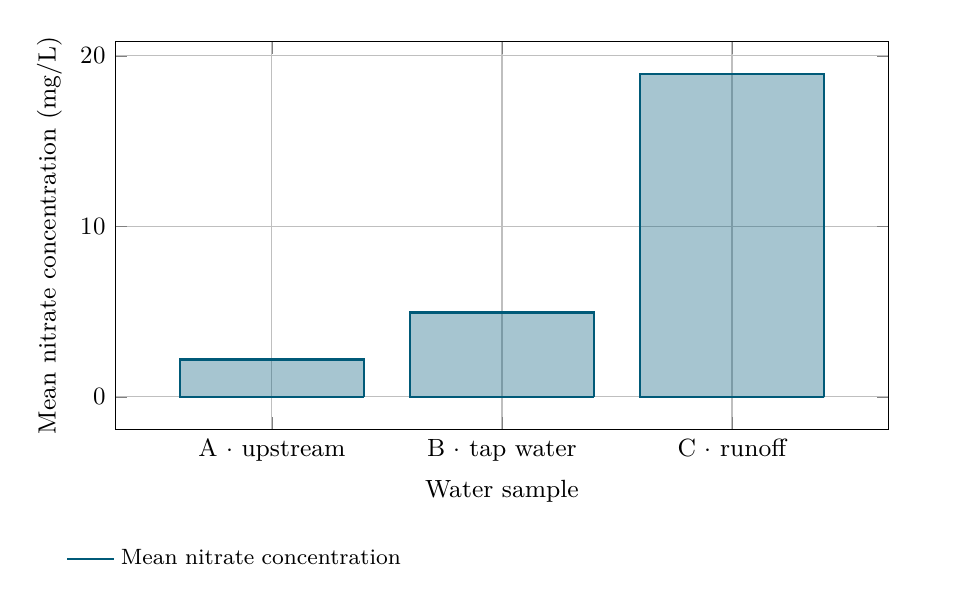
\begin{tikzpicture}
\begin{axis}[width=0.94\linewidth,
height=6.5cm,
scale only axis=false,
grid=major,
tick label style={font=\small},
label style={font=\small},
xlabel={Water sample},
ylabel={Mean nitrate concentration (mg/L)},
legend style={font=\footnotesize,draw=none,at={(0.5,-0.28)},anchor=north,legend columns=1,text width=0.85\linewidth,align=left},
unbounded coords=jump,
scaled ticks=false,
xtick={1,2,3},
xticklabels={{A \ensuremath{\cdot} upstream},{B \ensuremath{\cdot} tap water},{C \ensuremath{\cdot} runoff}}]
\addplot[color=pcd1,thick,fill=pcd1,fill opacity=0.35,mark=none] coordinates {(0.6,0) (0.6,2.2) (1.4,2.2) (1.4,0)} \closedcycle;
\addplot[color=pcd1,thick,fill=pcd1,fill opacity=0.35,forget plot,mark=none] coordinates {(1.6,0) (1.6,4.95) (2.4,4.95) (2.4,0)} \closedcycle;
\addplot[color=pcd1,thick,fill=pcd1,fill opacity=0.35,forget plot,mark=none] coordinates {(2.6,0) (2.6,18.925) (3.4,18.925) (3.4,0)} \closedcycle;
\addlegendentry{Mean nitrate concentration}

\end{axis}
\end{tikzpicture}
\end{center}
\par Sample C has the highest mean nitrate concentration.
\medskip

The scope of a conclusion follows the scope of the observations. Repeats from a prepared sample describe variation at the stages repeated in that procedure. Extending a statement to a lake, production batch or future sampling day calls for a sampling design that represents that target. Recording the preparation, measurement conditions and units keeps the numerical result connected to its chemical meaning.


\clearpage
\section{Build the analysis from description to modelling}
The course develops an analysis by adding tools to the same reasoning process. We first describe variables and observed values. We then summarize location, variation and distribution shape. Probability models connect these descriptions with questions about repeated sampling. Later methods use those foundations to compare groups, explain relationships and design informative experiments.


The roadmap in \hyperref[material-b5ce86c6cc6d0edf984904b455a3d1865147a744c3d57c70504f8c1219a74a6f]{Fig.~\ref*{material-b5ce86c6cc6d0edf984904b455a3d1865147a744c3d57c70504f8c1219a74a6f}} organizes these connections. Its steps are a route through related questions: what was measured, what pattern is present, how much variation is expected, and what conclusion does the evidence support? Earlier descriptions remain useful when a later model introduces additional assumptions.


\par\medskip
\Needspace{10cm}
\refstepcounter{figure}\label{material-b5ce86c6cc6d0edf984904b455a3d1865147a744c3d57c70504f8c1219a74a6f}
\noindent\textbf{Fig.~\ref*{material-b5ce86c6cc6d0edf984904b455a3d1865147a744c3d57c70504f8c1219a74a6f}.} Course roadmap connecting descriptive summaries, inference and modelling with analytical applications. Each step supplies tools for a different part of the measurement-to-decision process.\par\nopagebreak
\par\medskip\noindent\textcolor{pcd1}{\textbf{1. STATISTICAL FOUNDATIONS}}\par
Random variables \ensuremath{\cdot} mean values \ensuremath{\cdot} dispersion \ensuremath{\cdot} distributions

\par\noindent $\longrightarrow$ 2. builds on
\par\medskip\noindent\textcolor{pcd2}{\textbf{2. INFERENCE}}\par
Hypothesis testing \ensuremath{\cdot} t-tests \ensuremath{\cdot} ANOVA

\par\noindent $\longrightarrow$ 3. builds on
\par\medskip\noindent\textcolor{pcd3}{\textbf{3. REGRESSION + UNCERTAINTY}}\par
Models \ensuremath{\cdot} diagnostics \ensuremath{\cdot} confidence \ensuremath{\cdot} validation

\par\noindent $\longrightarrow$ 4. builds on
\par\medskip\noindent\textcolor{pcd4}{\textbf{4. DESIGN OF EXPERIMENTS}}\par
Effects \ensuremath{\cdot} interactions \ensuremath{\cdot} optimization

\par\noindent $\longrightarrow$ 5. builds on
\par\medskip\noindent\textcolor{pcd5}{\textbf{5. MULTIVARIATE ANALYSIS}}\par
Similarity \ensuremath{\cdot} clustering \ensuremath{\cdot} PCA

\par\noindent $\longrightarrow$ 6. builds on
\par\medskip\noindent\textcolor{pcd1}{\textbf{6. MACHINE LEARNING}}\par
Prediction \ensuremath{\cdot} classification \ensuremath{\cdot} validation


\medskip

Worked examples, discussion and executable calculations support complementary forms of learning. An example connects a calculation to a chemical situation. Discussion makes the choice of method and the interpretation explicit. Reproducing a calculation allows the observations and assumptions to be varied deliberately. A productive starting exercise is to name one analytical decision from your own work and list the measurements that would support it.


\end{document}
